\documentclass[conference]{IEEEtran}
\IEEEoverridecommandlockouts
\usepackage[T1]{fontenc}
\usepackage[utf8]{inputenc}
\usepackage{graphicx}
\usepackage{grffile}
\usepackage{hyperref}
\usepackage{amsmath}
\usepackage{listings}
\usepackage{url}

\title{Micro-MCP: A Microservice Architecture Pattern for the Model Context Protocol}

\author{\IEEEauthorblockN{Malik Abualzait}
\IEEEauthorblockA{\textit{Independent Researcher}\\
Email: malik.abualzait@example.com}}

\begin{document}
\maketitle

\begin{abstract}
The Model Context Protocol (MCP) is an emerging standard for exposing tools, resources, and prompts to large language models (LLMs) and agents. This paper introduces Micro-MCP, a microservice architecture pattern that composes many single-purpose MCP servers behind a lightweight gateway providing discovery, namespacing, policy enforcement, and audit. We motivate the pattern, define the threat and deployment models, describe a reference implementation, discuss security and operational considerations, compare with related approaches, and outline a path to production adoption.\footnote{Reference implementation: see repository README.}
\end{abstract}

\begin{IEEEkeywords}
Model Context Protocol, microservices, LLM, agents, gateway, security, policy, observability
\end{IEEEkeywords}

\section{Introduction}
LLM applications increasingly require controlled access to external tools and data. MCP\cite{mcp-wiki} provides a protocol for such access. However, monolithic MCP servers can entangle permissions, lifecycles, and blast radius, slowing iteration and complicating safety reviews. We propose Micro-MCP: decompose capabilities into small MCP services and compose them via a thin gateway. This separation improves isolation, deployability, and observability while retaining protocol compatibility and developer ergonomics.

\section{Background}
\subsection{Model Context Protocol}
MCP defines capabilities (tools, resources, prompts) and common transports using JSON-RPC\cite{jsonrpc}. Implementations exist in multiple languages. The protocol intentionally does not specify composition, discovery, or policy, leaving room for architectural patterns such as Micro-MCP.

\subsection{LLM Tool Use and Agentic Planning}
Recent work demonstrates that LLMs benefit from accessing external tools and structured context. ReAct combines reasoning and acting to iteratively call tools for decision making\cite{react}. Toolformer shows models can self-supervise to decide when and how to invoke APIs\cite{toolformer}. Gorilla studies instruction tuning for tool use and API grounding\cite{gorilla}. These lines of work motivate protocol-level, multi-capability access patterns such as MCP, and operational compositions such as Micro-MCP.

\subsection{Capability Model and Transports}
MCP exposes: (i) \emph{tools} with JSON-Schema\cite{jsonschema} input/output; (ii) \emph{resources} addressable via URIs; and (iii) \emph{prompts} as reusable templates. Transports include stdio for local development and network transports (e.g., WebSocket\cite{rfc6455}). JSON-RPC affords method invocation semantics, id correlation, and standard error categories.

\subsection{Microservices}
Microservices architectures advocate small, independently deployable services, often fronted by gateways and complemented by service meshes for cross-cutting concerns. Applied to MCP, each capability (e.g., filesystem access, HTTP fetching, vector search) is an independent MCP server, composed at the edge by a gateway rather than a mesh, due to the client-protocol nature of MCP.

\section{Motivation}
We identify three drivers: (1) security isolation and least privilege; (2) deployment agility and independent rollback; (3) operability via focused logging, metrics, and tracing (e.g., OpenTelemetry\cite{otel}).

\section{Architecture}
Micro-MCP consists of: (i) micro-MCP services exposing narrow MCP capabilities; (ii) a gateway that discovers services, merges capability catalogs, routes by namespace, enforces authentication and policy, and emits audit logs; and (iii) a registry or manifest for discovery.

\begin{figure}[t]
  \centering
  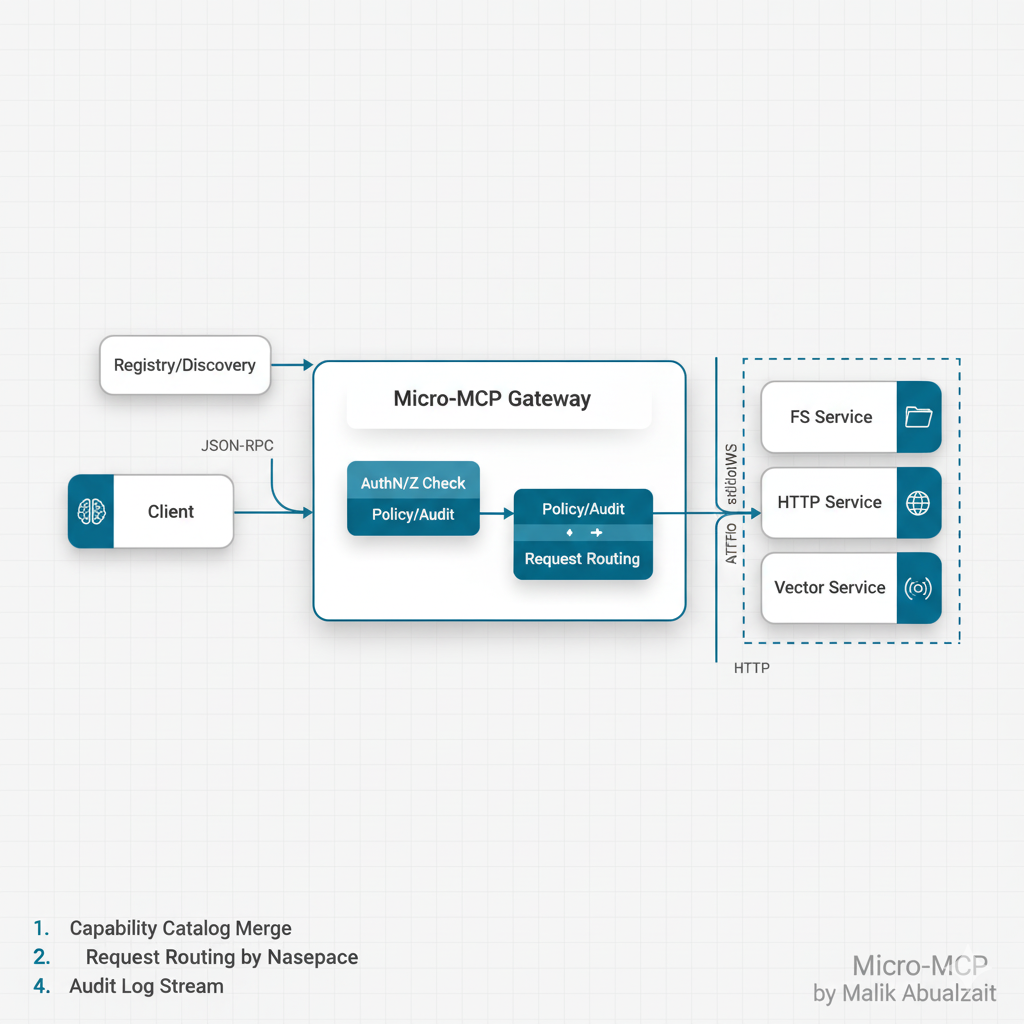
\includegraphics[width=0.48\textwidth]{figures/component-architecture-diagram.png}
  \caption{Micro-MCP components and flows.}
  \label{fig:components}
\end{figure}

\subsection{Data and Control Flow}
Requests from clients traverse the gateway for auth/policy, then route to services by namespace (e.g., \texttt{fs.listDir}). The gateway rewrites request identifiers for correlation, forwards to the target service, and restores client identifiers on response. Audit logs capture method, principal, decision, latency, and result category.

\section{Security and Policy}
Gateway authentication (e.g., static token for MVP, OpenID Connect in production\cite{oidc}) and allowlist/scopes enforce access, aligned with zero-trust principles\cite{nist-zt}. Attribute-based access control (ABAC)\cite{nist-abac} can express contextual decisions. Services use domain-scoped credentials (e.g., HTTP domain allowlist, read-only filesystem). Audit logs provide traceability; privacy-aware redaction and purpose binding are recommended for sensitive workloads.

\section{Reference Implementation}
We provide a runnable MVP with a Node.js gateway and three services: filesystem (list/read), HTTP fetcher (allowlisted domains), and vector search (naive cosine). The gateway uses stdio NDJSON JSON-RPC for simplicity and enforces a static token and allowlist policy. In production, we recommend WebSocket transports, containerized isolation, and signed artifacts.

\begin{figure}[t]
  \centering
  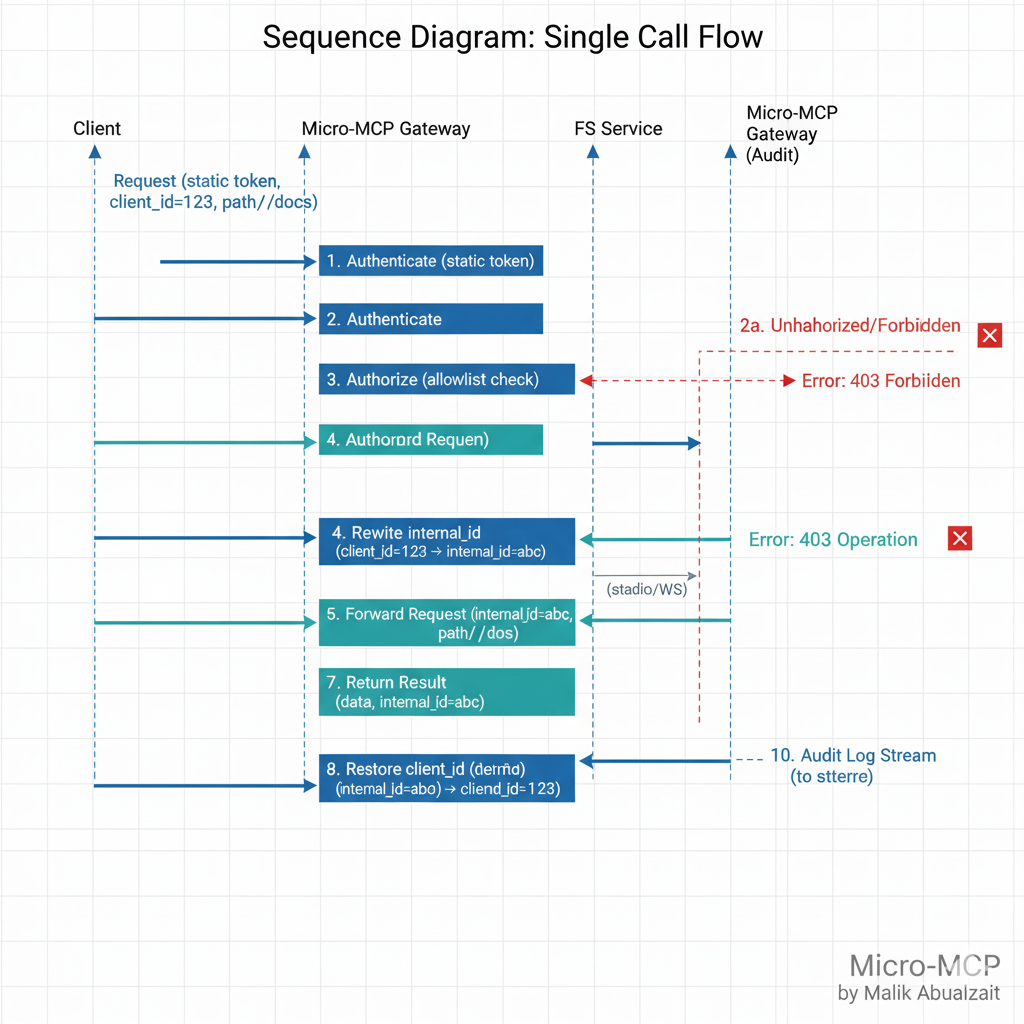
\includegraphics[width=0.48\textwidth]{figures/request-lifecycle-sequence-diagram.png}
  \caption{Request lifecycle through the gateway.}
  \label{fig:lifecycle}
\end{figure}

\section{Operational Considerations}
\subsection{Deployment}
Local development uses stdio and a static manifest; edge and cloud deployments can adopt WebSocket transports, containerized services, health checks, and autoscaling.

\subsection{Observability}
Structured audit logs at the gateway, per-service logs and health, and distributed tracing (Dapper\cite{dapper}, OpenTelemetry\cite{otel}) are recommended.

\section{Discussion}
We discuss namespacing and collision handling, caching immutable resources, and supply-chain hardening (SBOMs, signing). We also consider interop with existing agent tool ecosystems and argue for a capability catalog endpoint to improve discovery and documentation.

\section{Related Work and Literature Review}
Microservices surveys summarize benefits and challenges of decomposition and independent deployability\cite{dragoni-microservices, jamshidi-survey}. API gateways and service meshes address cross-cutting concerns in microservice systems; Istio\cite{istio} exemplifies mesh-side policy, observability, and resilience. Micro-MCP places analogous concerns at an MCP-aware gateway due to the client-session and capability-catalog needs of MCP. Service discovery and coordination foundations such as ZooKeeper\cite{zookeeper} inform registry design. Zero Trust\cite{nist-zt} informs authorization posture; ABAC\cite{nist-abac} frames contextual policy. Observability draws on large-scale tracing (Dapper\cite{dapper}) and open standards (OpenTelemetry\cite{otel}). On the LLM side, ReAct\cite{react}, Toolformer\cite{toolformer}, and Gorilla\cite{gorilla} motivate structured tool access. For software supply chain integrity, in-toto\cite{intoto} and TUF\cite{tuf} provide building blocks for artifact verification.

\section{Formalization and Threat Model}
\subsection{System Model}
We model services as a set \(S = \{s_1, \dots, s_n\}\), each offering a namespaced method set \(M_i\). The gateway provides a function \(R: (n, m, p) \mapsto s_i\) mapping namespace \(n\), method name \(m\), and parameters \(p\) to a target service. Policies are predicates \(P(n,m,\text{principal},\text{context})\rightarrow\{\top,\bot\}\).

\subsection{Adversary and Assumptions}
We assume network attackers (tampering, replay), compromised or buggy services, and misconfigured policies. The gateway is within the trust boundary but should be minimized and observable. We assume standard crypto channels for network transports and short-lived credentials for identities.

\subsection{Security Objectives}
Least privilege (scope minimization), blast radius containment, auditability, and policy transparency. Non-goals for MVP include end-to-end attestation and formal verification.

\section{Design Rationale}
We place composition at the gateway instead of a mesh because MCP sessions and capability catalogs are client-facing concerns. A gateway can enforce per-session policies, prompt for consent, and expose a consolidated catalog. Services remain small and focused, reducing cognitive and operational complexity.

\section{Interoperability}
Micro-MCP composes at the protocol boundary and therefore coexists with application-layer agent frameworks (e.g., LangChain\cite{langchain}, Semantic Kernel\cite{semantickernel}). Existing API gateways (Kong\cite{kong}, NGINX\cite{nginx}) can front the Micro-MCP gateway for TLS termination and coarse controls, while fine-grained capability policy remains protocol-aware inside the gateway. Policy engines such as OPA/Rego\cite{opa} or Cedar\cite{cedar} can externalize authorization decisions.

\section{Performance Considerations}
Per-call overhead includes gateway parsing, policy evaluation, and inter-process forwarding. Techniques include connection pooling, batching, backpressure, and caching of immutable resources. For large resources, signed URLs offload data transfer. Tracing enables latency attribution across the chain.

\section{Evaluation Plan}
We propose to evaluate: (i) security isolation by fault injection into one service; (ii) performance under increasing concurrency and payload sizes; (iii) developer productivity via time-to-add-capability; and (iv) policy correctness with conformance tests. Metrics include p50/p95 latency, error rates, policy decision times, and change lead time.

\section{Limitations}
The gateway is added complexity and a potential bottleneck. Services must adhere to schemas to retain strong typing. Discovery in the MVP is static; dynamic registries introduce their own consistency and availability trade-offs. Namespacing requires governance to avoid collisions.

\section{Future Work}
Standardized discovery metadata, dynamic health and version negotiation, richer policy (purpose binding, contextual ABAC), sandboxing and supply-chain hardening (SPDX\cite{spdx}, SLSA\cite{slsa}), and a capability catalog endpoint for clients.

\begin{figure}[t]
  \centering
  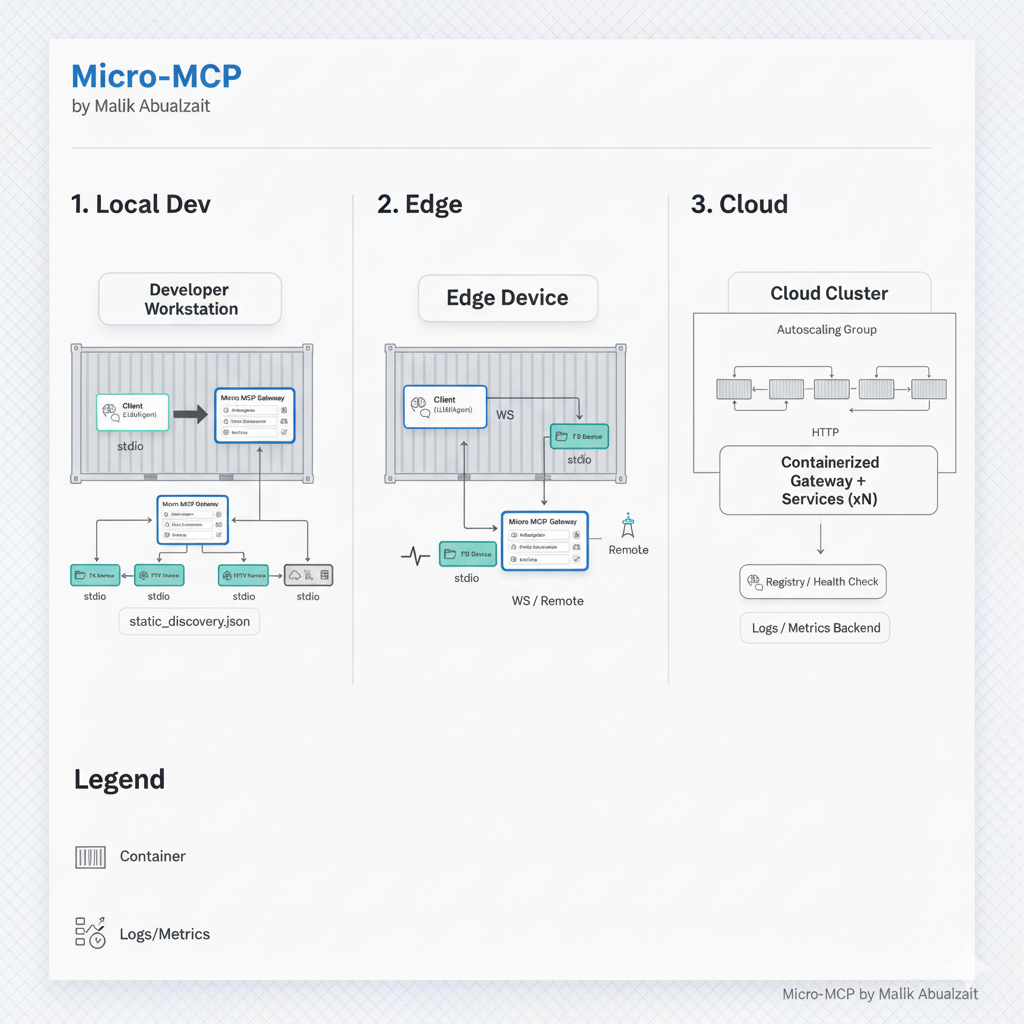
\includegraphics[width=0.48\textwidth]{figures/deployment-topology-local-edge-cloud.png}
  \caption{Deployment topologies: local, edge, and cloud.}
  \label{fig:deploy}
\end{figure}

\begin{figure}[t]
  \centering
  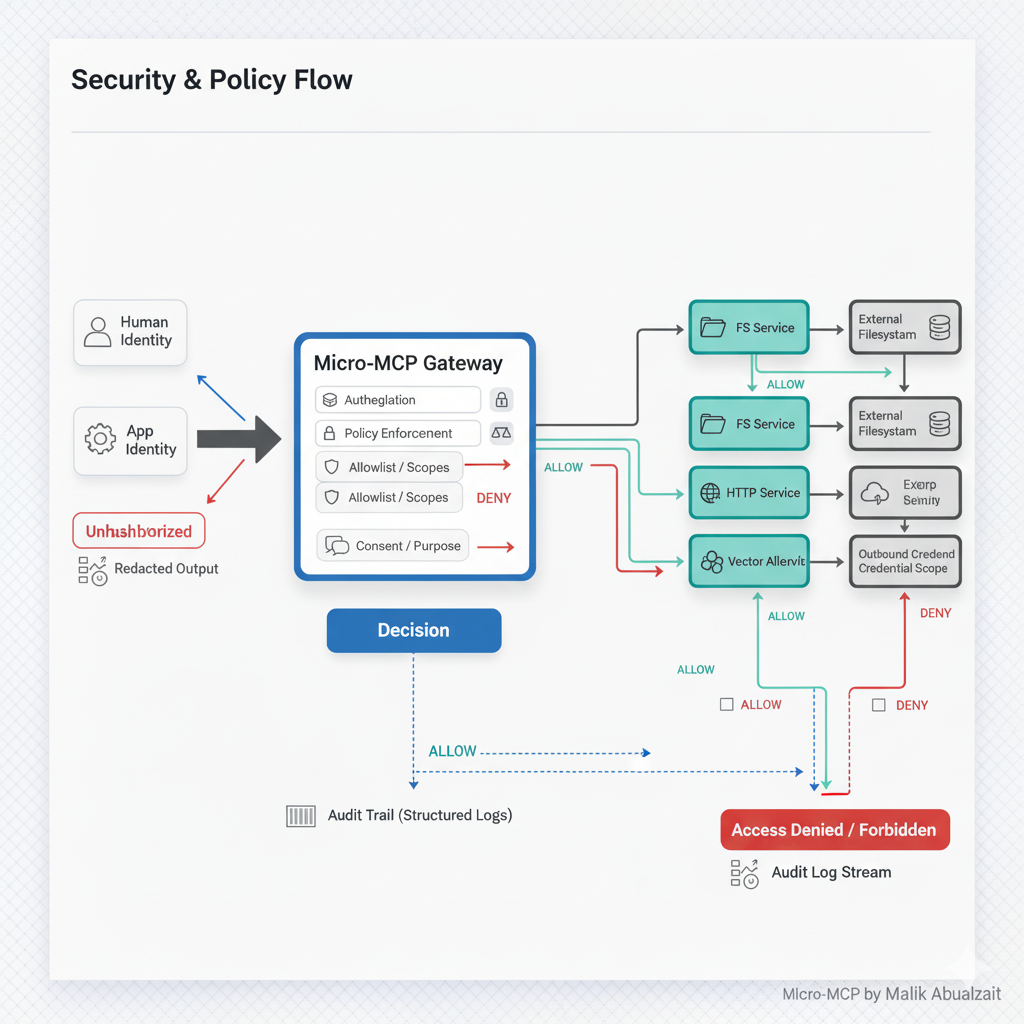
\includegraphics[width=0.48\textwidth]{figures/security-and-policy-flow.png}
  \caption{Security and policy flow across gateway and services.}
  \label{fig:security}
\end{figure}

\section{Conclusion}
Micro-MCP provides a practical path to adopt MCP in production with strong isolation and operability. Future work includes standardized discovery, richer policy, and reference deployments across environments.

\section*{Acknowledgments}
We thank early reviewers and the broader MCP community for discussions that informed this work.

\bibliographystyle{IEEEtran}
\bibliography{references}

\end{document}


